% \iffalse
\documentclass[journal,12pt,twocolumn]{IEEEtran}
\usepackage{cite}
\usepackage{amsmath,amssymb,amsfonts,amsthm}
\usepackage{algorithmic}
\usepackage{graphicx}
\usepackage{textcomp}
\usepackage{xcolor}
\usepackage{txfonts}
\usepackage{listings}
\usepackage{enumitem}
\usepackage{mathtools}
\usepackage{gensymb}
\usepackage{comment}
\usepackage[breaklinks=true]{hyperref}
\usepackage{tkz-euclide}
\usepackage{listings}
\usepackage{gvv}
\def\inputGnumericTable{}
\usepackage[latin1]{inputenc}
\usepackage{color}
\usepackage{array}
\usepackage{longtable}
\usepackage{calc}
\usepackage{multirow}
\usepackage{hhline}
\usepackage{ifthen}
\usepackage{lscape}
\usepackage{caption}

\newtheorem{theorem}{Theorem}[section]
\newtheorem{problem}{Problem}
\newtheorem{proposition}{Proposition}[section]
\newtheorem{lemma}{Lemma}[section]
\newtheorem{corollary}[theorem]{Corollary}
\newtheorem{example}{Example}[section]
\newtheorem{definition}[problem]{Definition}
\newcommand{\BEQA}{\begin{eqnarray}}
\newcommand{\EEQA}{\end{eqnarray}}
\newcommand{\define}{\stackrel{\triangle}{=}}
\theoremstyle{remark}
\newtheorem{rem}{Remark}
\begin{document}

\bibliographystyle{IEEEtran}
\vspace{3cm}

\title{NCERT 11.9.4 8Q}
\author{EE23BTECH11010 - Venkatesh D Bandawar $^{*}$% <-this % stops a space
}
\maketitle
% \newpage
\bigskip

\renewcommand{\thefigure}{\theenumi}
\renewcommand{\thetable}{\theenumi}

\textbf{Question:} Find the sum to $n$ terms of series , whose $n^{th}$ term is : $n(n+1)(n+4)$.

\textbf{Solution}
\begin{table}[!h] 
\centering
\begin{tabular}{|c|c|c|}
\hline
    Parameter & Description & Value\\
    \hline
    $P(s)$ & Plant Transfer Function & $\frac{0.001}{s\brak{\frac{s}{0.5}+1}\brak{\frac{s}{100}+1}}$\\
    \hline
    $C(s)$ & Lag Compensator  & $\frac{100\brak{\frac{s}{10}+1}}{\frac{s}{0.1}+1}$\\
    \hline
    $T(s)$ & Loop gain  & $P(s) C(s)$ \\
    \hline
    $\omega$ & Angular Frequency & 3rad/s \\
    \hline
\end{tabular}

\caption{Given parameters}
\label{given parameters list}
\end{table}

From equation \eqref{eq:11.9.5.26.2} to \eqref{eq:11.9.5.26.4},\\
    \begin{align}
        X(z) &= \frac{z^{-1}\brak{1+4z^{-1}+z^{-2}}}{\brak{1-z^{-1}}^4} + \frac{5z^{-1}\brak{z^{-1}+1}}{\brak{1-z^{-1}}^3} + \frac{4z^{-1}}{\brak{1-z^{-1}}^2} \cbrak{\abs{z}>1}\\
         Y(z) &= X(z)U(z)\\
         &=\frac{z^{-1}\brak{1+4z^{-1}+z^{-2}}}{\brak{1-z^{-1}}^5} + \frac{5z^{-1}\brak{z^{-1}+1}}{\brak{1-z^{-1}}^4} + \frac{4z^{-1}}{\brak{1-z^{-1}}^3} 
    \end{align}
    \begin{multline}
        = \frac{1}{4}\sbrak{\frac{z^{-1}\brak{1+11z^{-1}+11z^{-2}+z^{-3}}}{\brak{1-z^{-1}}^5}} \\
        +\frac{13}{6}\sbrak{\frac{z^{-1}\brak{1+4z^{-1}+z^{-2}}}{\brak{1-z^{-1}}^4}} + \frac{19}{4}\sbrak{\frac{z^{-1}\brak{1+z^{-1}}}{\brak{1-z^{-1}}^3}}\\
        + \frac{17}{6}\sbrak{\frac{z^{-1}}{\brak{1-z^{-1}}^2}} \cbrak{\abs{z}>1}
    \end{multline}
    where,
    \begin{align}
        n u(n) &\system{Z} \frac{z^{-1}}{\brak{1-z^{-1}}^2} \cbrak{\abs{z}>1} \label{eq:z transform of nu(n)} \\
        n^2 u(n) &\system{Z} \frac{z^{-1}\brak{1+z^{-1}}}{\brak{1-z^{-1}}^3} \cbrak{\abs{z}>1}\label{eq:z transform of n^2u(n)} \\
        n^3 u(n) &\system{Z} \frac{z^{-1}\brak{1+4z^{-1}+z^{-2}}}{\brak{1-z^{-1}}^4} \cbrak{\abs{z}>1}\label{eq:z transform of n^3u(n)} \\
        n^4 u(n) &\system{Z} \frac{z^{-1}\brak{1+11z^{-1}+11z^{-2}+z^{-3}}}{\brak{1-z^{-1}}^5} \cbrak{\abs{z}>1}\label{eq:z transform of n^4u(n)}
    \end{align}
    
    Taking reverse z transform, using equations \eqref{eq:z transform of nu(n)} to \eqref{eq:z transform of n^4u(n)}
    \begin{align}
        y(n) &= \brak{\frac{n^4}{4} + \frac{13n^3}{6} + \frac{19n^2}{4} + \frac{17n}{6}} u\brak{n}\\
        &= \brak{\frac{n^2\brak{n+1}^2}{4} + \frac{5n(n+1)(2n+1)}{6} 
        + \frac{4n(n+1)}{2}} u\brak{n}
    \end{align}
    \begin{figure}[!h] 
    \centering
    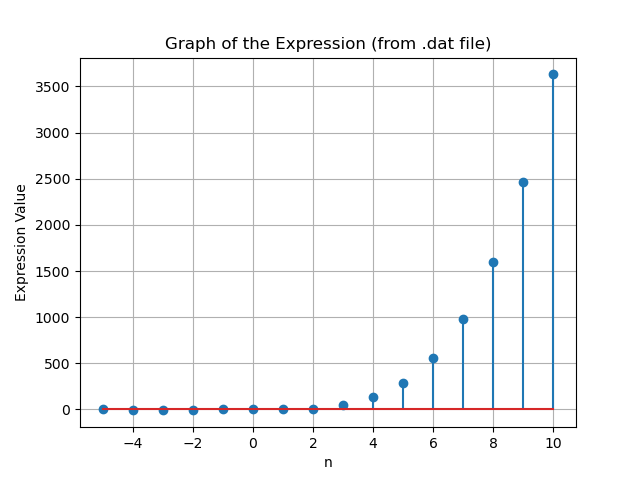
\includegraphics[width=\columnwidth]{figs/sumplot.png}
    \caption{Sum of n terms of series}
    \label{fig:Graph1_math.11.9.4.8}
    \end{figure}

\end{document}
